\section{Conclusion}
\label{sec:conclusion}
We analysed the simulation values, since they are more accurate than the theoretical analysis. However, the theoretical analysis was useful to guide us on what values to use in Ngspice. In spite of the relatively high cost, we achieved a voltage ripple of $3*10^{-5}V$ and an output voltage of 12V, which gave us a Merit Figure of 19.26.  This value shows that the goal of the lab assignment was achieved successfully.
All in all, this lab assignment showed us the challenges of a real project, because we were introduced to the concept of keeping a budget in mind while working on a solution to a problem. Once again, the outputs given by the predictions and the simulations differed considerably, and that can be seen as a consequence of the non-linear behavior of some of the components used (diodes). Also, the theoretical model used was the ideal one, which has some approximations in spite of giving consistent results.
\clearpage

\section{Side-by-side}
\label{sec:side-by-side}

\subsection{Envelope detector}
\begin{figure}[h] \centering
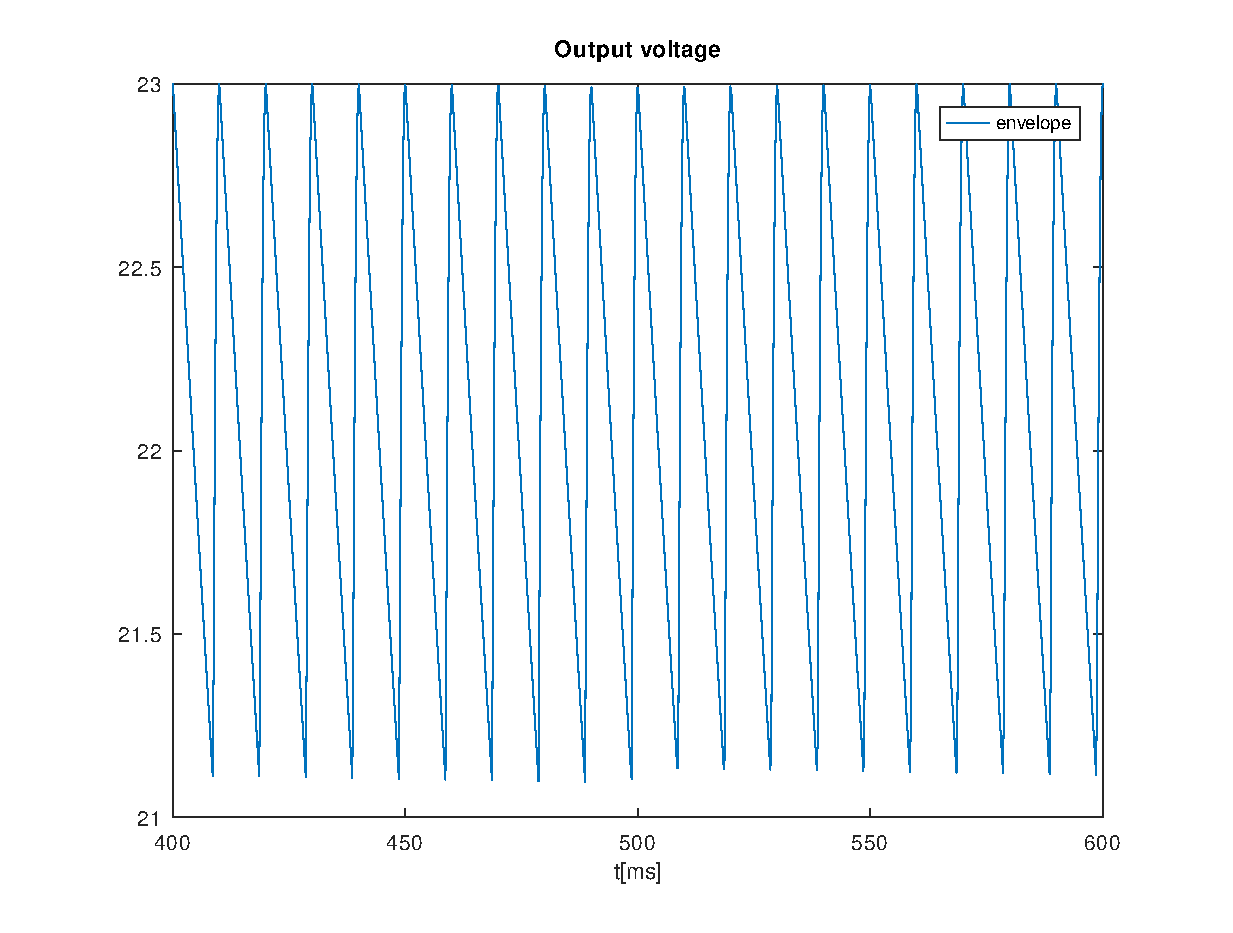
\includegraphics[scale=0.35]{vOenv_vOr.eps}
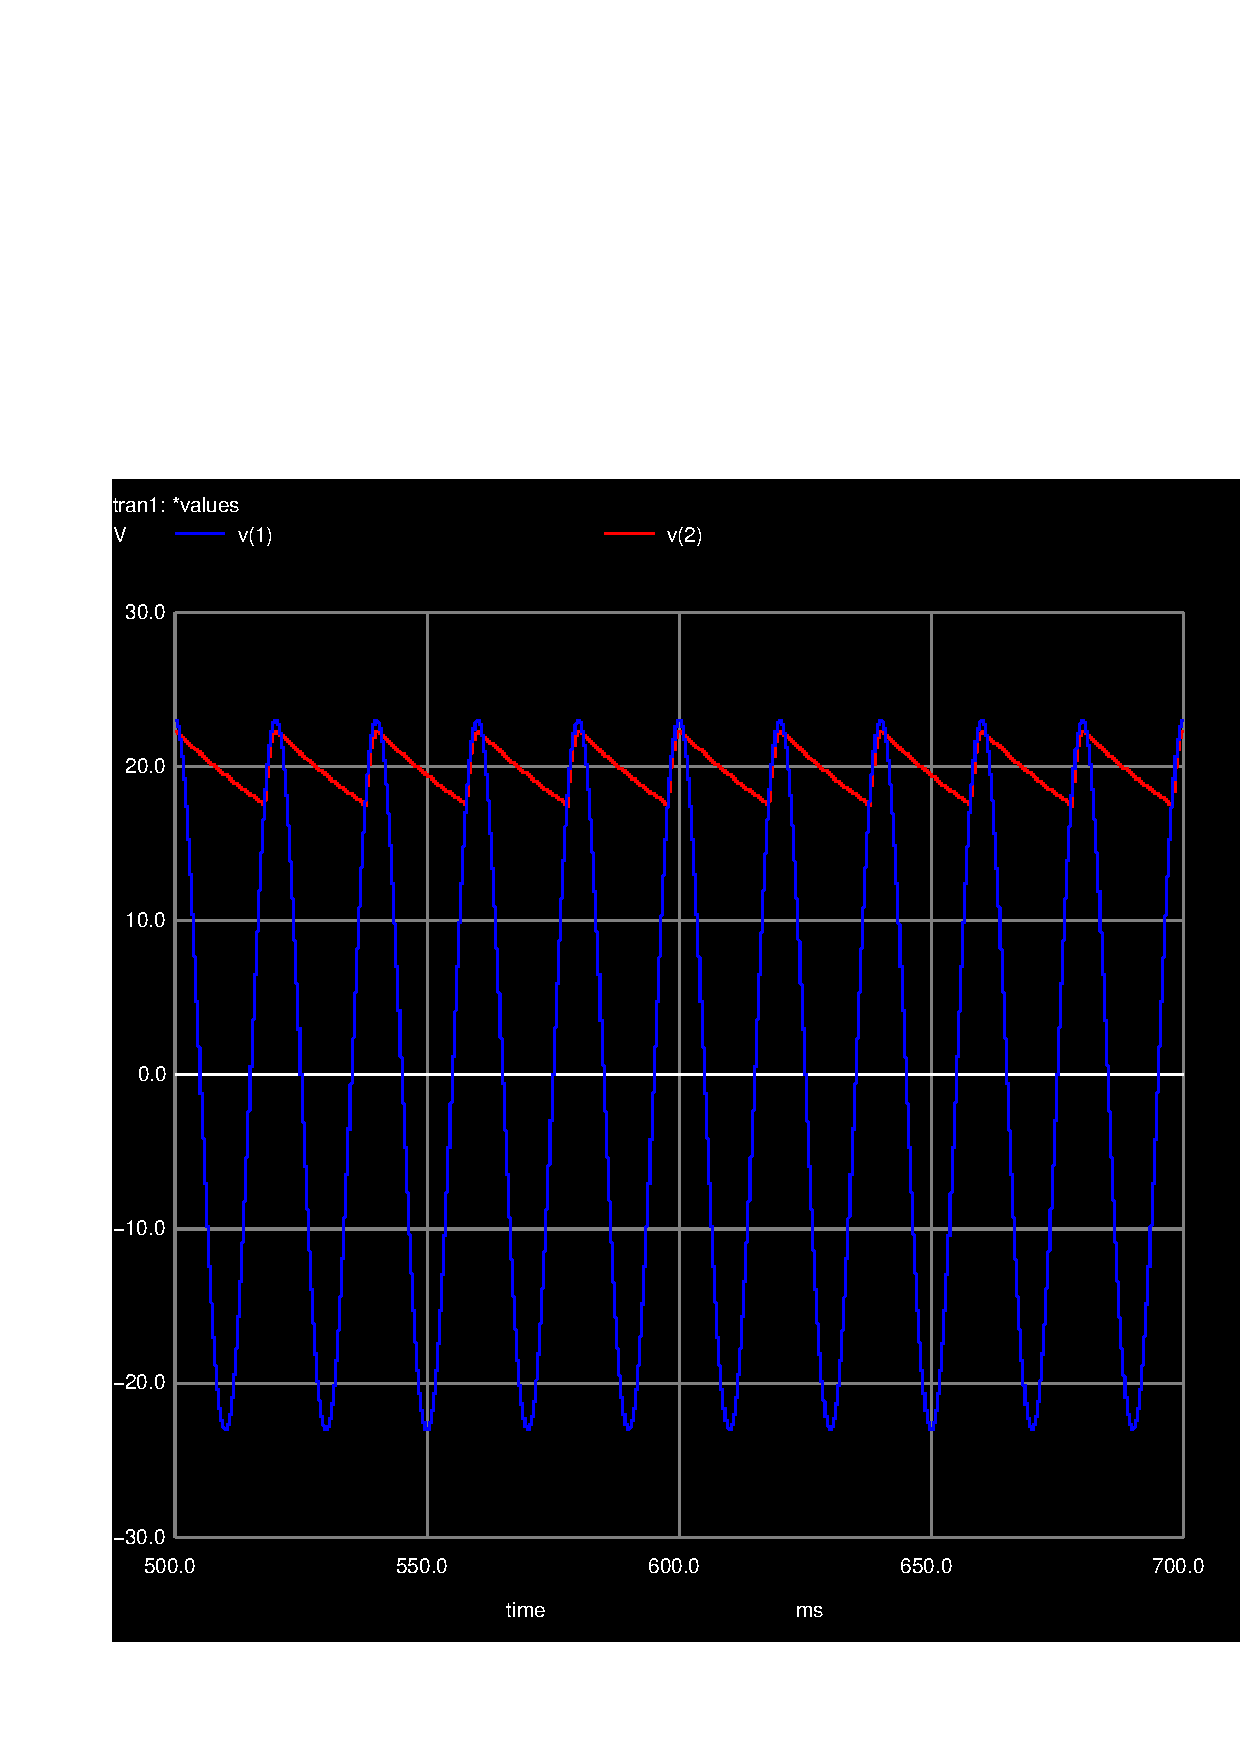
\includegraphics[scale=0.27]{ven.pdf}
\caption{Envelope detector}
\label{fig:comparison1}
\end{figure}
\FloatBarrier

\subsection{Voltage Regulator Output}
\begin{figure}[h] \centering
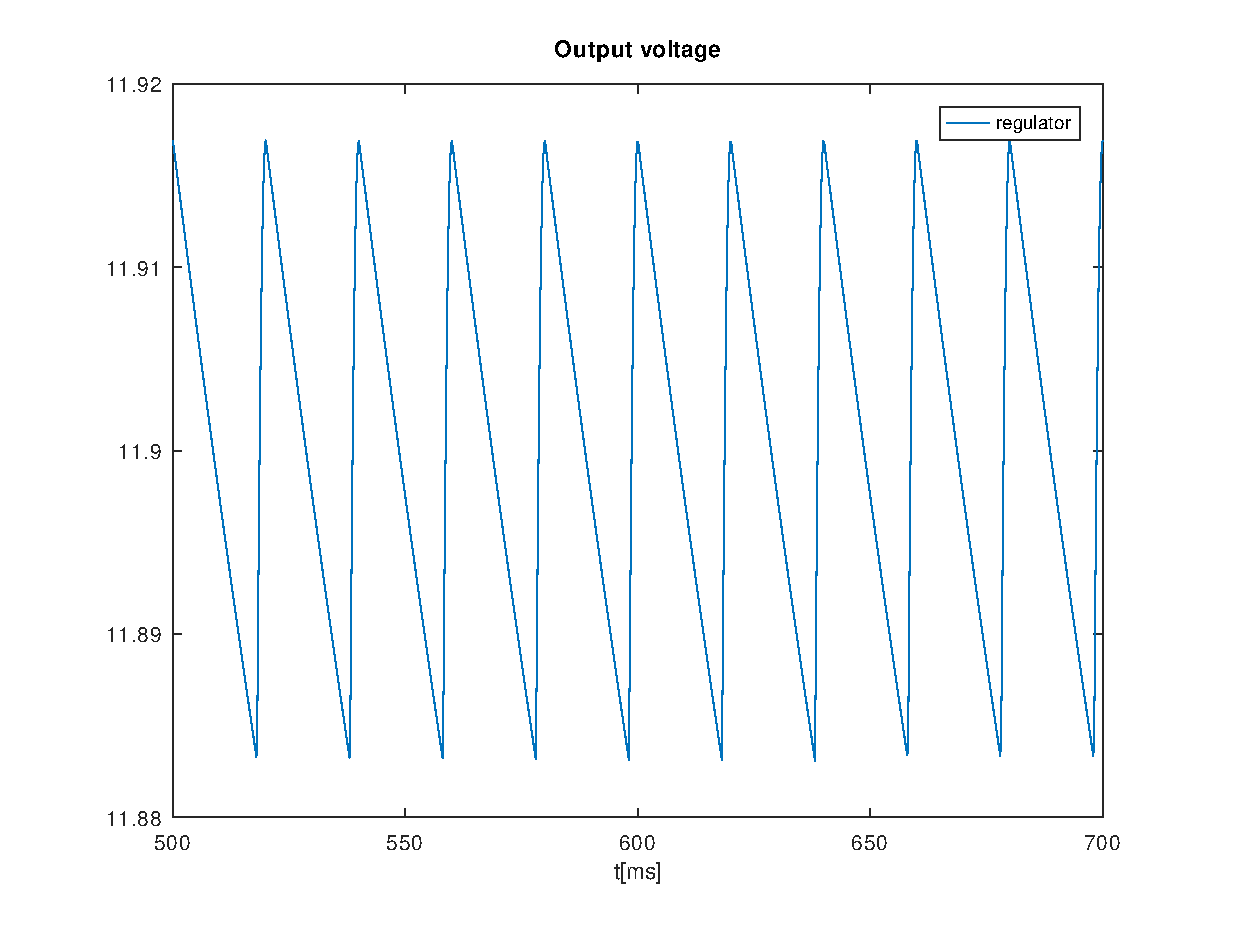
\includegraphics[scale=0.35]{vOreg.eps}
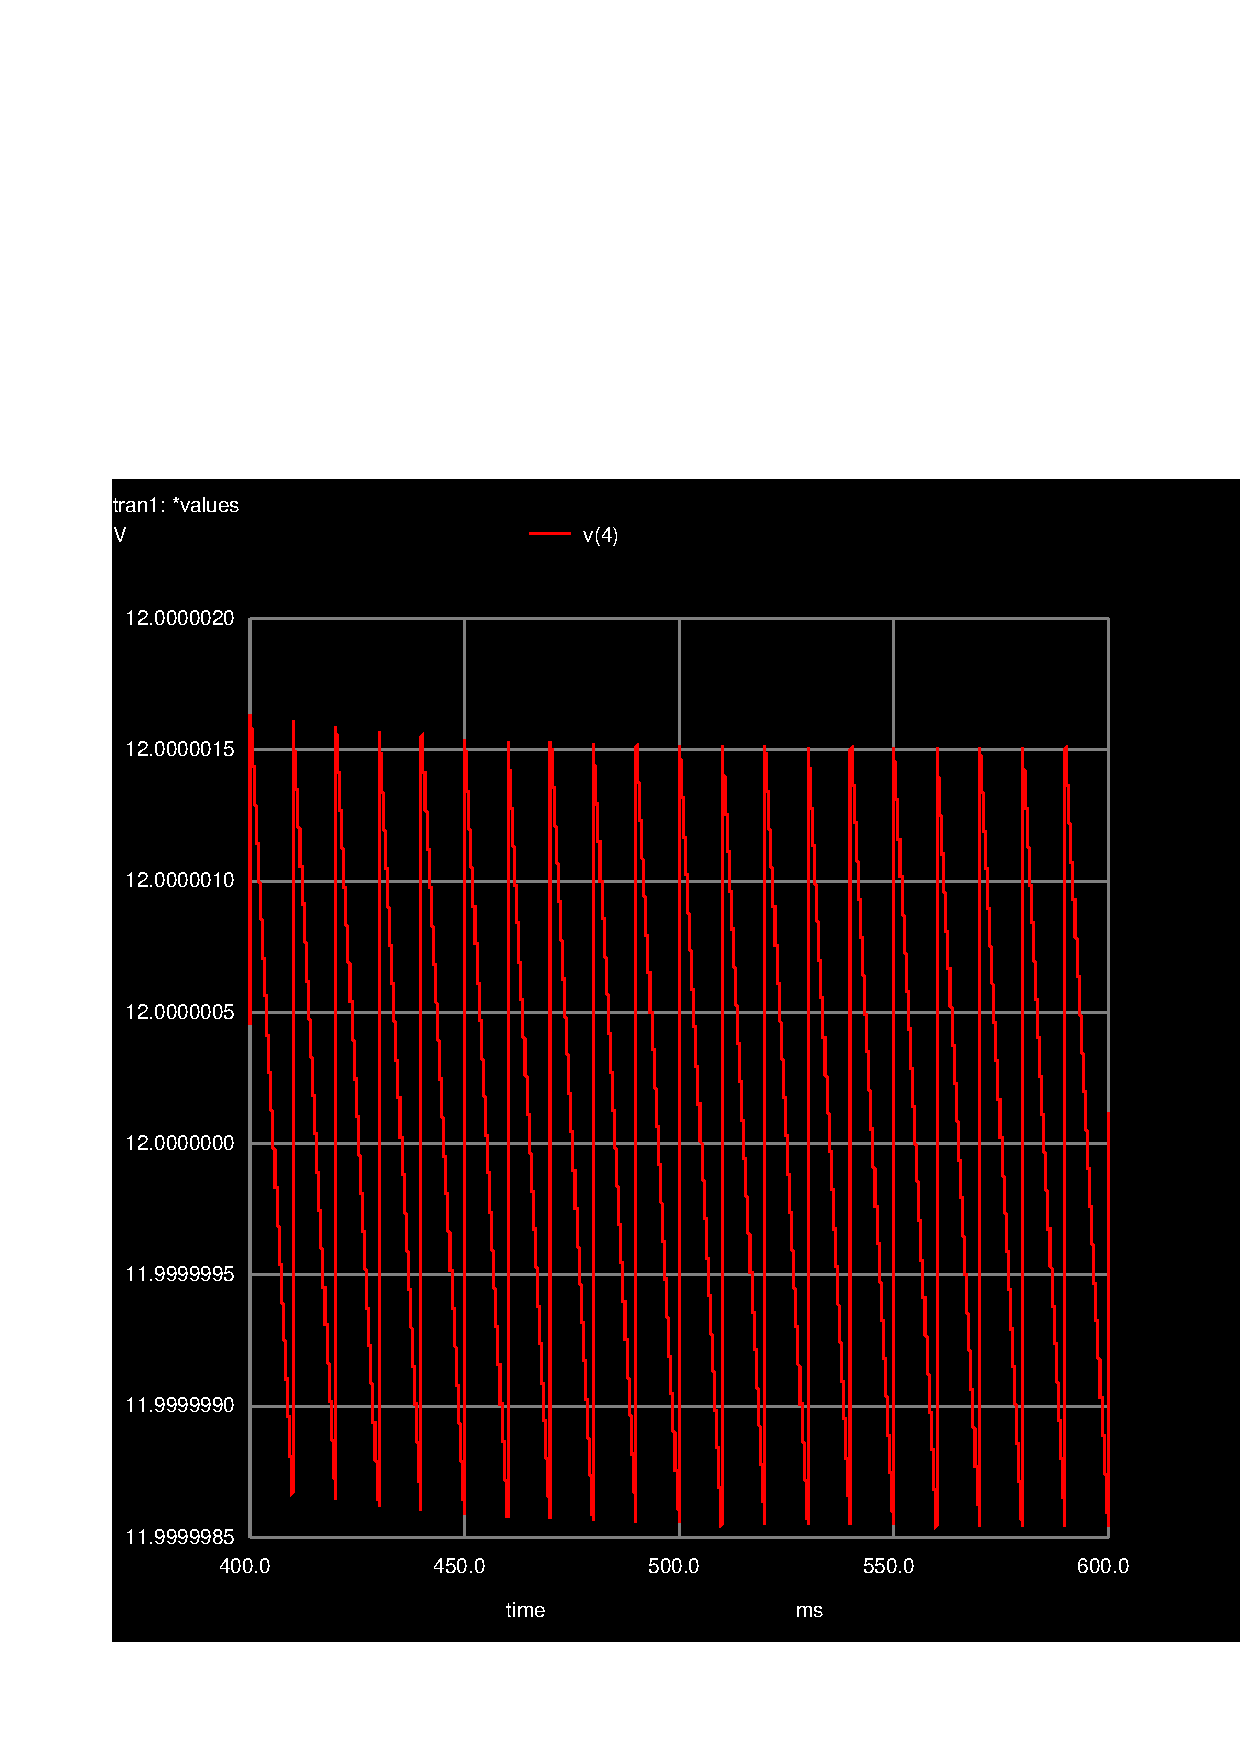
\includegraphics[scale=0.27]{vout.pdf}
\caption{Output voltage/Voltage Regulator Output}
\label{fig:comparison2}
\end{figure}
\FloatBarrier
\pagebreak

\subsection{vO Voltage Regulator - 12}
\begin{figure}[h] \centering
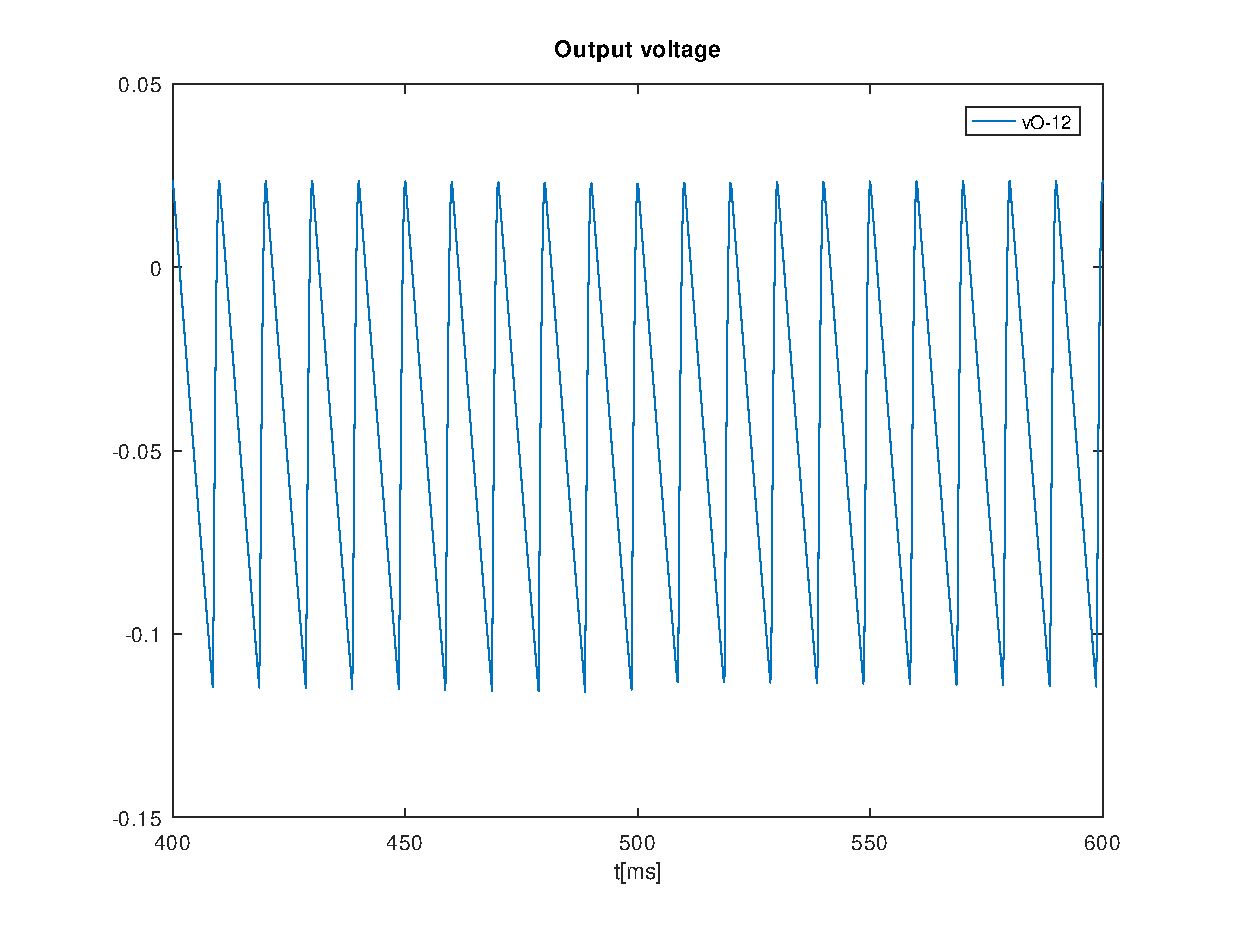
\includegraphics[scale=0.35]{vO-12.eps}
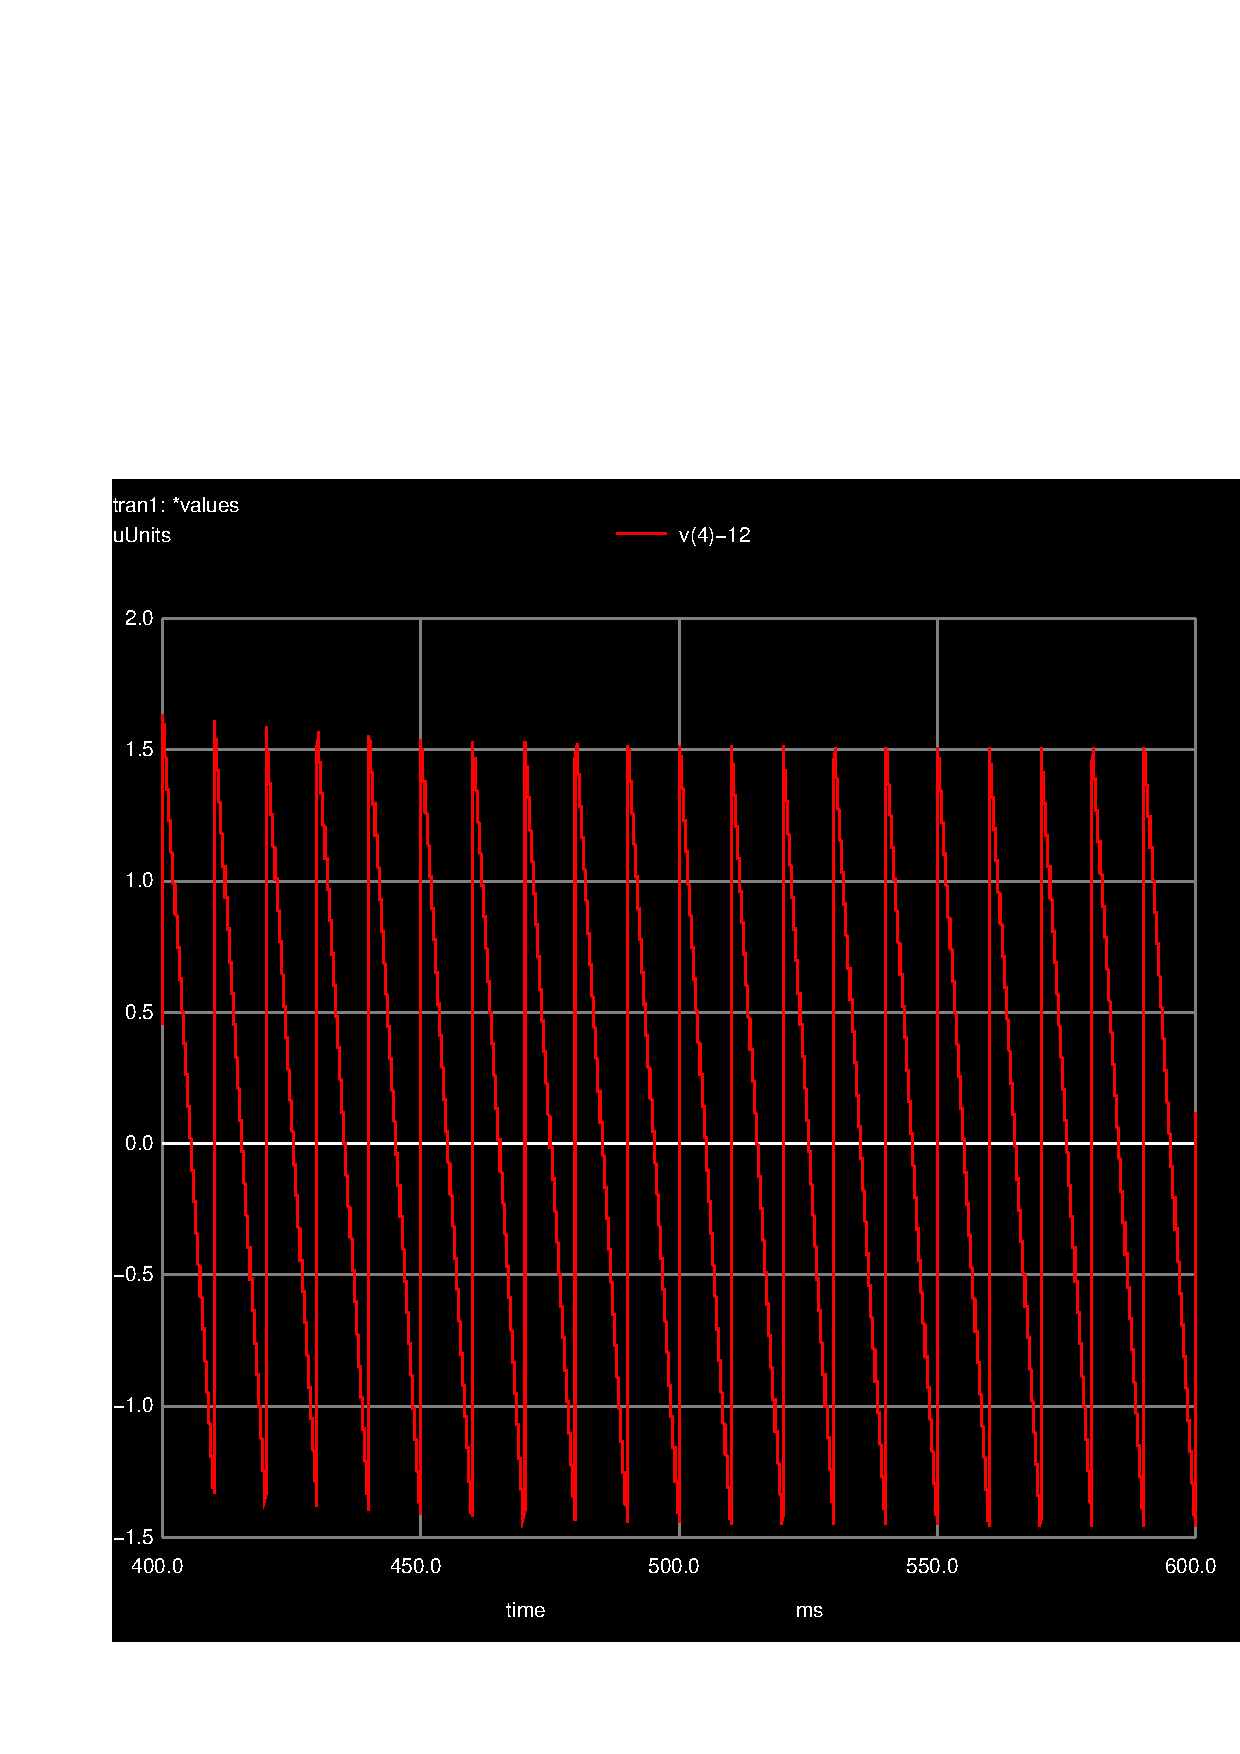
\includegraphics[scale=0.27]{vout-12.pdf}
\caption{vO Voltage Regulator - 12}
\label{fig:comparison3}
\end{figure}
\FloatBarrier
